\documentclass[final]{article}
%\usepackage[final]{graphics}
% final means "include the picture".  draft means "put a space with filename"
\usepackage[final]{graphicx}
\usepackage{latexsym}
\usepackage{amssymb}
\usepackage{amsmath}
\usepackage[normalem]{ulem}
% layout package provides the \layout command that shows page layout settings
\usepackage{layout}
% hyperref[1] provides ability to create hyperlinks
\usepackage{hyperref}
% framed provides an easy way to box a paragraph within a document
\usepackage{framed}
%\usepackage{showkeys}  %shows labels in margins see Gratzer p. 249
% these settings are mostly to make the margins smaller
\abovecaptionskip=0pt
\oddsidemargin=0pt
\textwidth=450pt
\textheight=650pt
\topmargin=-0.5in
\setlength{\marginparwidth}{0pt}
%  A tilde ‘~’ character generates a non-breaking space

\setlength{\parindent}{0cm} % no indent for paragraphs
\setlength{\parskip}{1.5ex} % more space between paragraphs.
\title{Curved Edge Physics}
\author{Erik Neumann\\
erikn@myphysicslab.com}
\date{September 4, 2015}
\begin{document}

\maketitle



%===============================================================
\section{Introduction}

We derive the physics of 2 dimensional rigid bodies with curved edges for calculating
contact forces in a rigid body physics engine. The cases handled are:

\begin{itemize}
  \item Vertex on Curved Edge
  \item Curved Edge on Straight Edge
  \item Curved Edge on Curved edge
\end{itemize}

We assume that the curved edge is circular for now, though that restriction can be
relaxed by finding the radius of curvature of the edge at the particular contact point.
That allows using these results for an oval shaped edge, for example.

We start from David Baraff's papers (see References \cite{dB94, dB97}) which handle the
Vertex on Straight Edge case. See also the summary on the \texttt{myphysicslab} website
at \url{http://www.myphysicslab.com/contact.html}.

The general idea is to develop an equation for the ``gap distance'' $d$ at the point of
contact. The gap distance is the distance between the two points on the bodies that are
in contact.

We then find the second derivative (acceleration) of the gap distance, $d''$. The
acceleration of the gap distance is the key quantity used to find the contact forces.
Terms from that gap acceleration equation will then go into the $\mathbf{A}$ matrix or
$\mathbf{b}$ vector that make up the matrix equation for contact forces. See the
references for more discussion.

\begin{figure}[ht]
    \centering
    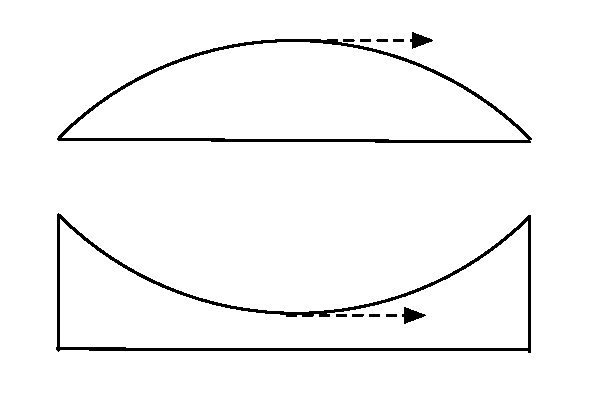
\includegraphics[width=0.45 \textwidth]{CEP_sliding_curved_edge.pdf}
    \caption{Vertex moving on curved edge}
    \label{fig:sliding_curved_edge}
\end{figure}

There are two main differences between curved edges and straight edges:

\begin{enumerate}

  \item For a curved edge, rotation about the center of curvature has no effect on the
  gap distance. This results in using the $\mathbf{U}$ vector to the center of curvature
  instead of the $\mathbf{R}$ vector to the point of impact (see section below on
  ``Implementation in Software'').

  \item Lateral movement along a curved edge (perpendicular to the normal) results in a
  change to the gap distance, just from the geometry of the curve. See
  Figure~\ref{fig:sliding_curved_edge}.

\end{enumerate}



%===============================================================
\section{Vertex on Straight Edge}

Here we review the ``Vertex on Straight Edge'' case, which is covered in the Baraff
paper \cite{dB94} and summarized at \url{http://www.myphysicslab.com/contact.html} (see
equations (5) and (6) on that web page).

\begin{figure}[ht]
    \centering
    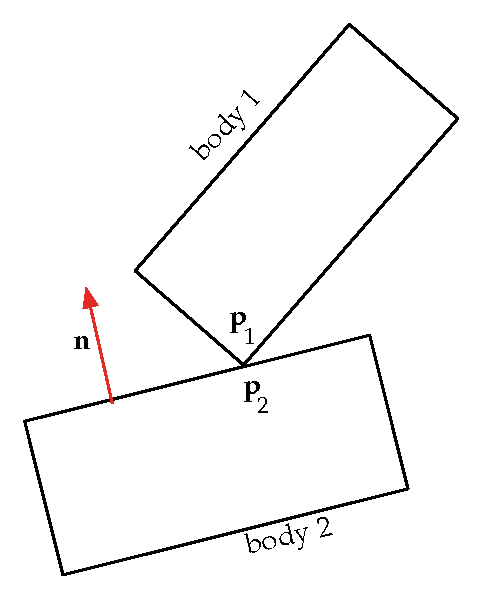
\includegraphics[width=0.45 \textwidth]{CEP_vertex_straight_edge.pdf}
    \caption{Two bodies in contact}
    \label{fig:two_bodies_in_contact}
\end{figure}

Let there be two bodies numbered 1 and 2, with body 2 specifying the normal vector
$\mathbf{n}$ pointing out from body 2 towards body 1, as shown in
Figure~\ref{fig:two_bodies_in_contact}. Let $\mathbf{p}_1$ be the point on body 1 that
is in contact with the point $\mathbf{p}_2$ on body 2. Let $d$ be the gap distance
between $\mathbf{p}_1$ and $\mathbf{p}_2$. Then we have

\begin{equation}\label{straight_vertex}
  d = \mathbf{n} \cdot (\mathbf{p}_1 - \mathbf{p}_2)
\end{equation}

We can now find the velocity and acceleration of the gap distance by taking derivatives
with respect to time.

\begin{equation}\label{straight_vertex_velocity}
  d' = \mathbf{n}' \cdot (\mathbf{p}_1 - \mathbf{p}_2)
      + \mathbf{n} \cdot (\mathbf{p}_1' - \mathbf{p}_2')
\end{equation}

\begin{equation}\label{straight_vertex_accel_1}
  d' = \mathbf{n}'' \cdot (\mathbf{p}_1 - \mathbf{p}_2)
      + 2 \mathbf{n}' \cdot (\mathbf{p}_1' - \mathbf{p}_2')
      + \mathbf{n} \cdot (\mathbf{p}_1'' - \mathbf{p}_2'')
\end{equation}

Because we are considering a point of contact, we have that $\mathbf{p}_1 - \mathbf{p}_2
= \mathbf{0}$ so the above simplifies to

\begin{equation}\label{straight_vertex_accel_2}
  d'' = 2 \mathbf{n}' \cdot (\mathbf{p}_1' - \mathbf{p}_2')
      + \mathbf{n} \cdot (\mathbf{p}_1'' - \mathbf{p}_2'')
\end{equation}

On the page \url{http://www.myphysicslab.com/contact.html} we go on to explain how the
velocity dependent parts of $d''$ go into the $\mathbf{b}$ vector, and we calculate how
each contact force affects the gap acceleration $d''$ which is how the $\mathbf{A}$
matrix is formed.



%===============================================================
\section{Vertex on Circular Edge}

\begin{figure}[ht]
    \centering
    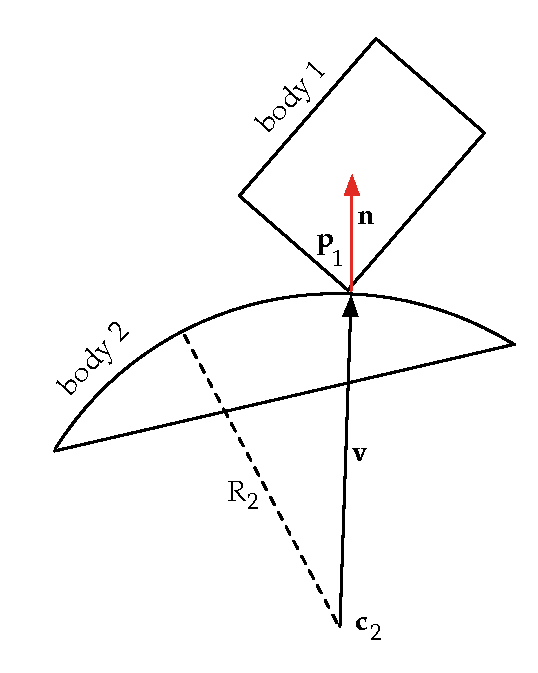
\includegraphics[width=0.45 \textwidth]{CEP_vertex_circle_edge.pdf}
    \caption{Vertex on circular edge}
    \label{fig:vertex_on_circle}
\end{figure}

Let $\mathbf{p}_1$ be the vertex on body 1 that is in contact with the circular edge on
body 2. Let $\mathbf{c}_2$ be the center of the circular edge on body 2; let $R_2$ be
the radius of the circular edge. See Figure~\ref{fig:vertex_on_circle}. Then the
distance gap between the two bodies is

\[
  d = \mathbf{n} \cdot (\mathbf{p}_1 - \mathbf{c}_2) - R_2
\]

For the circular edge, the normal follows the vertex $\mathbf{p}_1$ and we can define it
as the normalized direction vector from the center to the point:

\[
  \mathbf{n} = \frac { \mathbf{p}_1 - \mathbf{c}_2 } { \|\mathbf{p}_1 - \mathbf{c}_2\| }
\]

Let $\mathbf{v} = \mathbf{p}_1 - \mathbf{c}_2$, then

\begin{equation}\label{vertex_circle_normal}
  \mathbf{n} = \frac{ \mathbf{v} } { \| \mathbf{v} \| }
\end{equation}

\begin{equation}\label{vertex_circle_gap}
  d = \mathbf{n} \cdot \mathbf{v} - R_2 = \mathbf{v} \cdot
    \frac{ \mathbf{v} } { \| \mathbf{v} \| } - R_2 = \| \mathbf{v} \| - R_2
\end{equation}

where we used the identity

\[
  \| \mathbf{v} \| = \sqrt{ \mathbf{v} \cdot \mathbf{v} }
\]

Assuming that the radius of the circular edge does not change, we take derivative with
respect to time.

\begin{equation}\label{deriv_mag_v}
  d' =  \| \mathbf{v} \| '
  = \frac{ d } { d t} \sqrt{ \mathbf{v} \cdot \mathbf{v} }
  = \frac {1}{2} (\mathbf{v} \cdot \mathbf{v}) ^{-\frac{1}{2}}
  (\mathbf{v} \cdot \mathbf{v}' + \mathbf{v}' \cdot \mathbf{v})
  = \frac{ \mathbf{v} \cdot \mathbf{v}' } { \| \mathbf{v} \| }
  = \mathbf{n} \cdot \mathbf{v}'
\end{equation}

\begin{framed}

  Another way to get the same result is to start again with equation
  (\ref{vertex_circle_gap}) and take the first derivative

  \[
    d = \mathbf{n} \cdot \mathbf{v} - R_2
  \]

  \[
    d' = \mathbf{n}' \cdot \mathbf{v} + \mathbf{n} \cdot \mathbf{v}'
  \]

  The derivative of the normal is perpendicular to the normal (see appendix), so:

  \[
    \mathbf{n}' \cdot \mathbf{v} = 0
  \]

  because the dot product of two perpendicular vectors is zero. Therefore we get to the
  same result as equation (\ref{deriv_mag_v}).

\end{framed}

Take derivative of equation (\ref{deriv_mag_v}) to get acceleration:
\[
  d'' = \mathbf{n}' \cdot \mathbf{v}' + \mathbf{n} \cdot \mathbf{v}''
\]

Or equivalently

\begin{equation}\label{accel_vertex_circle}
  d'' = \mathbf{n}' \cdot (\mathbf{p}_1' - \mathbf{c}_2')
    + \mathbf{n} \cdot (\mathbf{p}_1'' - \mathbf{c}_2'')
\end{equation}

Comparing this to the ``Vertex/Straight Edge'' equation (\ref{straight_vertex_accel_2})
we see there is a factor of 2 difference in the velocity term, and we are looking at the
movement of the center of the circle rather than the movement of the point on the
circular edge.



%===============================================================
\section{Straight/Circular Edge}

\begin{figure}[ht]
    \centering
    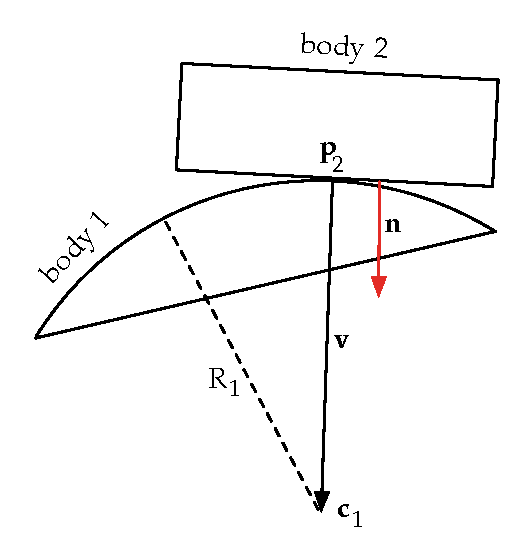
\includegraphics[width=0.45 \textwidth]{CEP_straight_circle_edge.pdf}
    \caption{Straight edge on circular edge}
    \label{fig:straight_circle_edge}
\end{figure}

In the case of a contact point between a straight edge and a circular edge, we regard
the normal as being rigidly attached to the straight edge.

Let $\mathbf{n}$ be the normal from the straight edge on body 2, let $\mathbf{p}_2$ be a
point on the straight edge, let $\mathbf{c}_1$ be the center of the circular edge on
body 1, and let $R_1$ be the radius of the circular edge. See
Figure~\ref{fig:straight_circle_edge}.

The gap distance is

\[
  d = \mathbf{n} \cdot (\mathbf{c}_1 - \mathbf{p}_2) - R_1
\]

Let $\mathbf{v} = \mathbf{c}_1 - \mathbf{p}_2$, then

\[
  d = \mathbf{n} \cdot \mathbf{v}  - R_2
\]

\[
  d' = \mathbf{n}' \cdot \mathbf{v} + \mathbf{n} \cdot \mathbf{v}'
\]

\begin{equation}\label{straight_circle_accel}
  d'' = \mathbf{n}'' \cdot \mathbf{v} + 2 \mathbf{n}' \cdot \mathbf{v}'
      + \mathbf{n} \cdot \mathbf{v}''
\end{equation}

Unlike the ``Vertex/Straight Edge'' case, the first term doesn't disappear because
$\mathbf{v}$ is non zero in this case. The other terms are handled similarly to the
Vertex/Straight Edge case, except that we look at the velocity and acceleration of the
center of the circle instead of the contact point on the circle.

The normal vector doesn't change magnitude, only direction, and we know it is rotating
at with angular velocity $\omega_2$. Let $\vec{\omega}_2 = (0, 0, \omega_2)$ be the
vector perpendicular to the 2D plane representing the angular velocity of the straight
edge body. Then the derivatives of the normal vector are:

\[
  \mathbf{n}' = \vec{\omega}_2 \times \mathbf{n}
\]

\[
  \mathbf{n}'' = \vec{\omega}_2 \times \vec{\omega}_2 \times \mathbf{n}
               = - \omega_2^2 \mathbf{n}
\]

Because the gap is assumed to be of size zero at the moment of contact, we have that

\[
  d = 0 = \mathbf{n} \cdot \mathbf{v} - R_1
\]

\[
  \mathbf{n} \cdot \mathbf{v} = R_1
\]

The normal acceleration term from (\ref{straight_circle_accel}) is velocity dependent,
so it goes in the $\mathbf{b}$ vector.

\[
  \mathbf{n}'' \cdot \mathbf{v} = - \omega_2^2 \mathbf{n} \cdot \mathbf{v}
    = - \omega_2^2 R_1
\]

The acceleration is then

\begin{equation}\label{straight_circle_accel_2}
  d'' =  2 \mathbf{n}' \cdot \mathbf{v}'
      + \mathbf{n} \cdot \mathbf{v}'' - \omega_2^2 R_1
\end{equation}

Or equivalently:

\begin{equation}\label{straight_circle_accel_3}
  d'' =  2 \mathbf{n}' \cdot (\mathbf{c}_1' - \mathbf{p}_2')
      + \mathbf{n} \cdot (\mathbf{c}_1'' - \mathbf{p}_2'') - \omega_2^2 R_1
\end{equation}



%===============================================================
\section{Circular/Circular Edge}

\begin{figure}[ht]
    \centering
    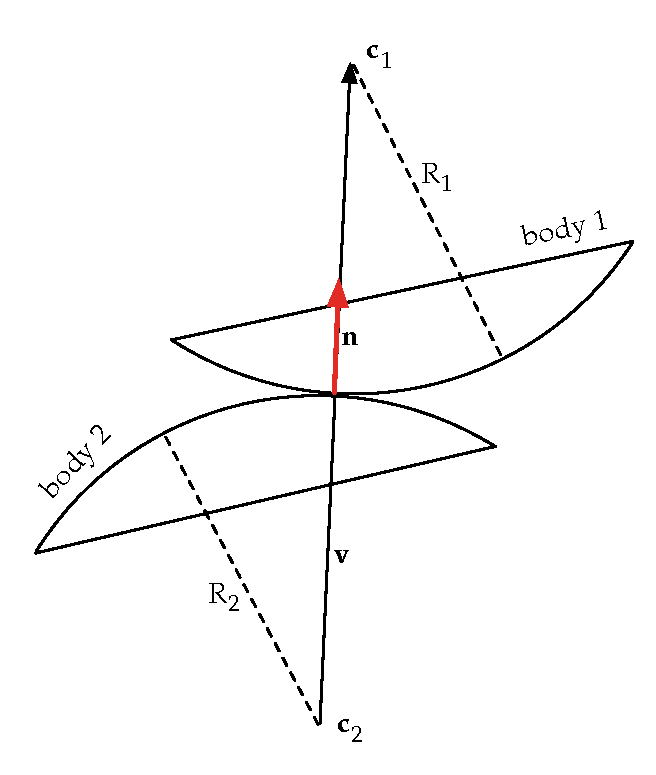
\includegraphics[width=0.45 \textwidth]{CEP_circle_circle_edge.pdf}
    \caption{Two circular edges in contact}
    \label{fig:circle_circle_edge}
\end{figure}

Here we consider a contact point between two circular edges. This case is similar to the
``Vertex/Circular Edge'' case, except that the vertex is replaced by the center of the
other circle.

Let $\mathbf{n}$ be the normal from the edge on body 2 at the contact point. Let
$\mathbf{c}_1$ and $\mathbf{c}_2$ be the centers of the circular edges on body 1 and 2
respectively. Let $R_1$, $R_2$ be the radius of the circular edges on body 1 and body 2.
See Figure~\ref{fig:circle_circle_edge}.


Let $\mathbf{v} = \mathbf{c}_1 - \mathbf{c}_2$.

The normal points in the same direction as $\mathbf{v}$:

\[
  \mathbf{n} = \frac { \mathbf{v} } { \|\mathbf{v}\| }
\]

The gap distance is given by:

\[
  d = \mathbf{n} \cdot \mathbf{v} - (R_1 + R_2)
\]

The first derivative is

\[
  d' = \mathbf{n}' \cdot \mathbf{v} + \mathbf{n} \cdot \mathbf{v}'
\]

The first term is zero because the derivative of the normal is perpendicular to the
normal (see appendix) and the normal is parallel to $\mathbf{v}$, therefore:

\[
  d' = \mathbf{n} \cdot \mathbf{v}'
\]

The second derivative is

\[
  d'' = \mathbf{n}' \cdot \mathbf{v}' + \mathbf{n} \cdot \mathbf{v}''
\]

or equivalently

\begin{equation}\label{accel_circle_circle}
  d'' = \mathbf{n}' \cdot (\mathbf{c}_1' - \mathbf{c}_2')
    + \mathbf{n} \cdot (\mathbf{c}_1'' - \mathbf{c}_2'')
\end{equation}



%===============================================================
\section{Implementation in Software}

\begin{figure}[ht]
    \centering
    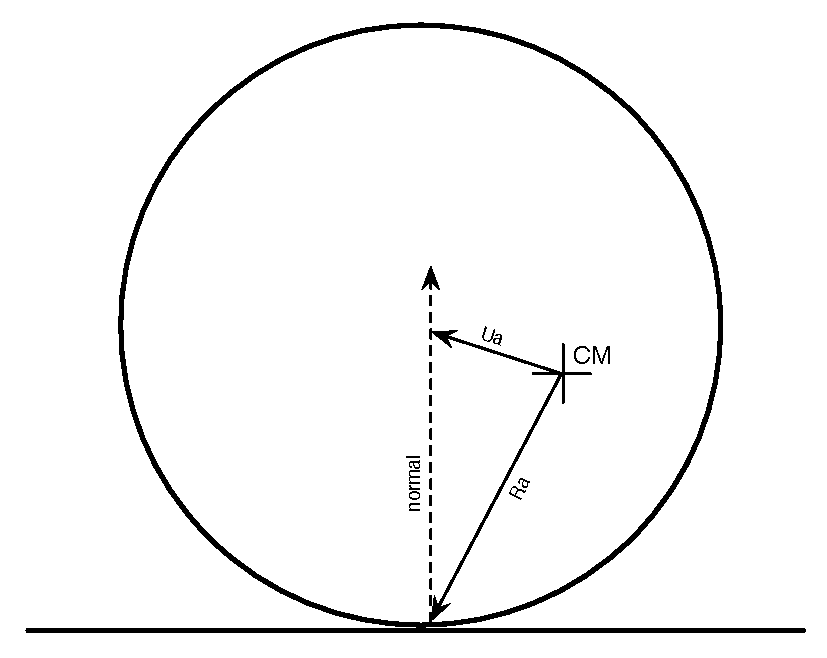
\includegraphics[width=0.6 \textwidth]{CEP_Equiv_U_R_Vectors.pdf}
    \caption{$\mathbf{U}$ and $\mathbf{R}$ Vectors for Curved Edge}
    \label{fig:CEP_Equiv_U_R_Vectors}
\end{figure}

In the myphysicslab software, we find the movement of the center of the circular edge by
looking at the $\mathbf{U}$ vector which goes from the center of mass to the center of
the circular edge, see Figure~\ref{fig:CEP_Equiv_U_R_Vectors}. This is in contrast to
looking at the $\mathbf{R}$ vector which goes from center of mass to the point of
contact, which is used for the ``Vertex/Straight Edge'' case.

This use of the $\mathbf{U}$ vector can be seen in the software that

\begin{itemize}

  \item sets up the $\mathbf{A}$ matrix which captures the effect of forces on the
    acceleration of the center of the circle

  \item sets up the $\mathbf{b}$ vector which captures the velocity dependent terms

\end{itemize}

Additionally, the various cases (Vertex/Curved, Straight/Curved, Curved/Curved) each
have the different factors derived above, and these can be seen in the software that
calculates the $\mathbf{b}$ vector.




%===============================================================
\section{Appendix}

Proof that derivative of a normal is perpendicular to the normal:

By definition, a normal is of constant unit length. Assume it is rotating at rate
$\omega$ at the current moment. Then we can write an equation for the normal
$\mathbf{n}$

\[
\mathbf{n} = [cos(\omega t + a), sin(\omega t + a)]
\]

where $t$ is time and $a$ is a constant.  Taking derivative with respect to time:

\[
\mathbf{n}' = [-\omega sin(\omega t + a), \omega cos(\omega t + a) ]
\]

which is $\omega$ times a vector perpendicular to $\mathbf{n}$



%===============================================================
\section{References}

\begin{thebibliography}{9}
\bibitem{dB94}
  David Baraff,
  \emph{Fast Contact Force Computation for Nonpenetrating Rigid Bodies},
  Computer Graphics Proceedings, Annual Conference Series, 1994; pages 23-34.

\bibitem{dB97}
  David Baraff,
  \emph{An Introduction to Physically Based Modeling: Rigid Body Simulation
  II - Nonpenetration Constraints},
  Siggraph '97 Course Notes.

\bibitem{eN15}
  Erik Neumann,
  \emph{myphysicslab website} has a summary of the Baraff paper at\\
  \url{http://www.myphysicslab.com/contact.html}.

\end{thebibliography}

% layout package provides the \layout command that shows page layout settings
%\layout


\end{document}
